\section{Theorie}
\label{sec:Theorie}
\subsection{Bestzung im Atom}
Die innersten Schalen eines Atoms sind, nach dem Pauli-Prinzip, vollständig mit Elektronen besetzt.
Die äußeren Schalen hingegen folgen einer temperaturabhängigen Verteilung.
Im thermischen Gleichgewicht gilt für zwei Zustände mit den Energien $W_\mathrm{1}$ und $W_\mathrm{2}$ nach der Boltzmann-Verteilung:
\begin{align}
  \frac{N_2}{N_2}=\frac{g_\mathrm{2}}{g_\mathrm{1}}\frac{\exp(-W_\mathrm{2}/kT)}{\exp(-W_\mathrm{1}/kT)}.
\end{align}
Hierin sind $g_1$ und $g_2$ statistische Gewichte, die angeben wie viele Zustände zu den Energien $W_\mathrm{1}$ bzw. $W_\mathrm{2}$.

\subsection{Energienivau-Struktur}
Aus der Quantenmechanik ist bekannt, dass der Gesamtdrehimpuls $J=\vec{L}+\vec{S}$,
mit $\vec{L}$d dem Bahndrehimpuls und $\vec{S}$ der Eigendrehimpuls, an ein magnetisches Moment $\vec{\mu_\mathrm{J}}$
koppelt:
\begin{align}
  \vec{\mu_\mathrm{J}}=-g_\mathrm{J}\mu_\mathrm{B}\vec{J}.
\end{align}
Hierbei sind $g_\mathrm{J}$ der Landé-Faktor und $\mu_\mathrm{B}$ das Bohrsche Magneton.
Mit dem vektoriellen Zusammenhang vom magnetischen Moment mit dem Drehimpuls, sowie
geometrischen Betrachtungen ergibt sich der Landé-Faktor zu:
\begin{align}
  g_\mathrm{J}=\frac{3,0023J(J+1)+1,0023[S(S+1)-L(L+1)]}{2J(J+1)}.
\end{align}
Im externen Magnetfeld verschieben sich die Energieniveaus, bedingt durch  die Wechselwirkung des magnetischen
Moments mit dem Magnetfeld. Für die Energiebilanz ist nur die Z-Komponente $\vec{\mu_\mathrm{J}}(\vec{Z}||\vec{B})$ des magnetischen Moments
entscheidend.
Für die Energie gilt dann:
\begin{align}
  U_\mathrm{mag}=M_\mathrm{J}g_\mathrm{J}\mu_\mathrm{B}B,
\end{align}
mit $M_\mathrm{J}$ als Orientierungsquantenzahl mit dem Wertevorrat:
\begin{align}
  -J,-J+1,...,0,...,J-1,J.
\end{align}
Die Aufspaltung in die sich ergebenden $2J+1$ UnterNiveaus nennt sich Zeemann-Aufspaltung.

Unter der Annahme eines hinreichend schwachen, äußeren Magnetfeldes und eines Kernspins ungleich null, kann eine Kopplung des Gesamtdrehipulses $\vec{J}$ der
Elektronenhülle an den Kernspin $\vec{I}$ beobachtet werden. Es ergibt sich der Gersamtdrehimpuls $\vec{F}=\vec{I}+\vec{J}$.
Die entstehende Aufspaltung nennt sich Hyperfeinstruktur.
Die Anzahl der Hyperfeinstrukturterme ist gleich $2J+1$ oder $2I+1$, jenachdem ob $J<I$ oder $J>I$ ist.
Die Terme werden durch die Quantenzahl $F$ unterschieden, welche von $I+J$ bis $|I-J|$ läuft.
Beim Anlegen eines Magnetfeldes spalten sich die HyperfeinstrukturNiveaus zusätzlich in $2F+1$-Zeeman-Niveaus auf, mit der Quantenzahl $M_\mathrm{F}$
welche von $-F$ bis $F$ läuft.
Für die Energiedifferenz der Zeeman-Niveaus gilt dann:
\begin{align}
  U_\mathrm{HF}=g_\mathrm{F}\mu_\mathrm{F}B.
\end{align}
Mit $g_\mathrm{F}$ als Landé-Faktor:
\begin{align}
  g_\mathrm{F}=g_\mathrm{J}\frac{F(F+1)+J(J+1)-I(I+1)}{2F(F+1)}.\label{eqn:JI}
\end{align}

\subsection{Optisches Pumpen}
Optisches Pumpen ist die Inversion der Energiezustände eines Atoms, durch optische Anregung.
Es folgt eine Erläuterung anhand eines hypothetischen Alkali-Atoms.
\begin{figure}
    \centering
    \includegraphics[width=0.5\textwidth]{Uebergang.PNG}
    \caption{Zeeman-Aufspaltung des hyphotetischen Alkali-Atoms und die möglichen Übergänge.\cite{skript}}
    \label{fig:Uebergang}
\end{figure}

In Abbildung \ref{fig:Uebergang} sind mögliche Übergänge dargestellt, diese lassen sich folgendermaßen nach der Polarisation der Strahlung kategorisieren:
\begin{itemize}
  \item{$\sigma^+$-Übergang: Der Spin ist antiparallel zur Ausbreitungsrichtung der Lichtquanten, dies entspricht rechtszirkular-polarisiertem Licht ($\Delta M_\mathrm{J}=+1$)}
  \item{$\sigma^-$-Übergang: Der Spin ist parallel zur Ausbreitungsrichtung der Lichtquanten, dies entspricht linkszirkular-polarisiertem Licht ($\Delta M-\mathrm{J}=-1$)}
  \item{$\pi$-Übergang: Linerar-polarisiertes Licht ($\Delta M_\mathrm{J}=0$)}.
\end{itemize}
Angenommen das Alkali-Atom wird mit rechtszirkular-polarisiertem Licht bestrahlt, so werden Elektronen des $^2S_\mathrm{\frac{1}{2}}$ Niveaus mit $M_\mathrm{J}=-\frac{1}{2}$
angeregt und
gehen über in das $^2P_\mathrm{\frac{1}{2}}$ mit $M_\mathrm{J}=+\frac{1}{2}$. Durch die sogenannte spontane Emission findet ein Rückgang sowohl ins
 $^2S_\mathrm{\frac{1}{2}}$ Niveaus mit $M_\mathrm{J}=+\frac{1}{2}$ als auch ins $^2S_\mathrm{\frac{1}{2}}$ Niveaus mit $M_\mathrm{J}=-\frac{1}{2}$ statt,
da aber die Anregung nur im $^2S_\mathrm{\frac{1}{2}}$ Niveau mit $M_\mathrm{J}=-\frac{1}{2}$ erfolgt, leert sich dieses Nivau.
Die gewünschte Inversion der Energiezustände tritt ein.\\
Eine weitere Methode die Elektronen in den Grundzustand zu bekommen nennt sich induzierte Emission.
Bei dieser Methode wird ein Photon mit einer Energie gleich dem Energieabstand zwischen dem $^2S_\mathrm{\frac{1}{2}}$ Niveau mit $M_\mathrm{J}=+\frac{1}{2}$
und  $M_\mathrm{J}=-\frac{1}{2}$ eingestrahlt. Dadurch kehrt das Elektron zurück in
den Grundzustand und es werden zwei Photonen mit gleicher Energie emittiert.\\
Beide Arten der Emission, bildlich dargestellt in Abbildung \ref{fig:emission}, laufen parallel ab, jedoch dominiert die induzierte Emission gegenüber der spontanen.
Deren Übergangswahrscheinlichkeit ist um den Faktor $5,5\cdot10^{25}$ größer. Die induzierte Emission kann dazu genutzt werden die Zeeman-Niveaus auszumessen.
\begin{figure}
    \centering
    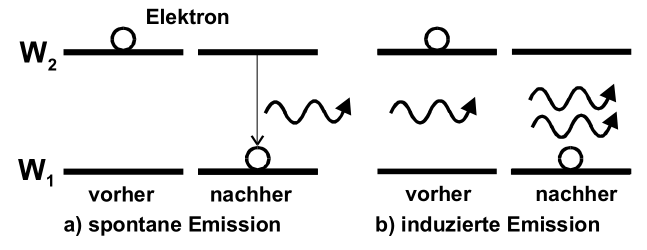
\includegraphics[width=0.5\textwidth]{emission.PNG}
    \caption{Die beiden Arten der Emission.\cite{skript}}
    \label{fig:emission}
\end{figure}

\subsection{Präzisionsmessung der Zeeman-Aufspaltung}
Eine mit dem zu untersuchenden Material gefüllte Dampfzelle ist nach abgeschlossenem Pumpvorgang transparent.
Wird ein variables Hochfrequenzfeld angelegt und ein Magnetfeld durchfahren, so setzt die Inversion der Besetzungszahlen in den S-Niveaus ein. Die Transparenz
beginnt. Sobald das Magnetfeld den Wert:
\begin{align}
  B_\mathrm{m}=\frac{4\pi m_\mathrm{0}}{e_\mathrm{0}g_\mathrm{F}}\nu \label{eqn:keineahnung}
\end{align}
erreicht, startet die induzierte Emission und das obere S-Niveau wird
entleert. Weil das untere Nivau zum Teil wieder gefüllt ist, kann das
eingestrahlte $\sigma^+$-Licht erneut absorbiert werden.
Im Resonanzfall nimmt die Transparenz ab, dies ist in Abbildung \ref{fig:Transparenz}
dargestellt.
\begin{figure}
    \centering
    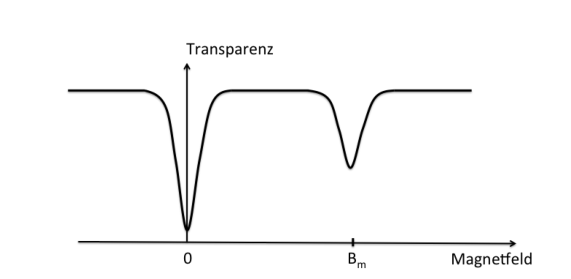
\includegraphics[width=0.5\textwidth]{transparenz.PNG}
    \caption{Die Transparenz einer Dampfzelle für $\sigma^+$-Licht in Abhängigkeit vom Magnetfeld
    bei konstantem Hochfrequenzfeld.\cite{skript}}
    \label{fig:Transparenz}
\end{figure}

\subsection{Quadratischer Zeeman-Effekt}
Bei höheren Flussdichten müssen für die Übergangsenergien die höheren Ordnungen von $B$ berücksichtigt werden. Nach Breit-Rabi gilt:
\begin{align}
  U_\mathrm{HF}=g_\mathrm{F}\mu_\mathrm{B}B+ g^2_\mathrm{F}\mu^2_\mathrm{B}B^2\frac{(1-2M_\mathrm{F})}{\Delta E_\mathrm{Hy}}
\end{align}
Die Zeeman-Aufspaltung ist bei höheren Magnetfeldern abhängig von der Hyperfeinstruktur. Dies wird als quadratischer Zeeman-Effekt bezeichnet.
